\section{Roboterfunktionen}
\subsection{Grosser Roboter}

\begin{frame}
	\frametitle{Grosser Roboter}
	\framesubtitle{Supportrad}
	\begin{columns}
		\begin{column}{0.42 \textwidth}
			\begin{itemize}
				\item nicht benötigt
			\end{itemize}
		\end{column}
		\begin{column}{0.58 \textwidth}
			\vspace{-2.8em}
			\begin{figure}[h]
				\centering
				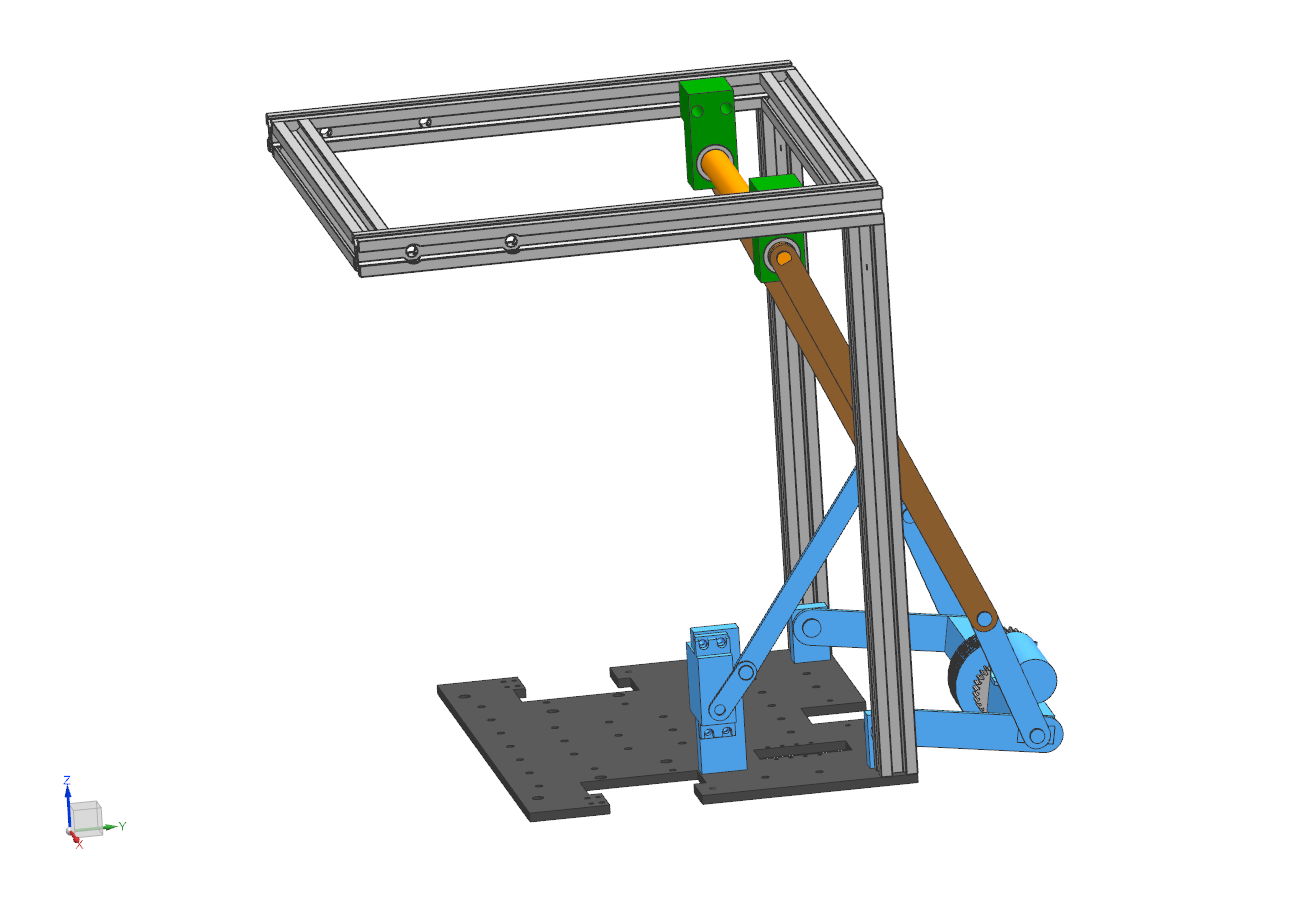
\includegraphics[width = 1 \textwidth]{../images/presentation/supportrad.png}
			\end{figure}
		\end{column}
	\end{columns}
\end{frame}

\begin{frame}
	\frametitle{Grosser Roboter}
	\framesubtitle{Walze und Leitplanke}
	\begin{columns}
		\begin{column}{0.6 \textwidth}
			\begin{itemize}
				\item Aufnahme der \textit{Titanium Ores}
				\item Spielelemente dürfen nicht beschäditgt werden
				\item Gummibänder und Kabelbinder
				\item Bereichsvergrösserung durch Leitplanken
			\end{itemize}
		\end{column}
		\begin{column}{0.4 \textwidth}
			\vspace{-2.5em}
			\begin{figure}[h]
				\centering
				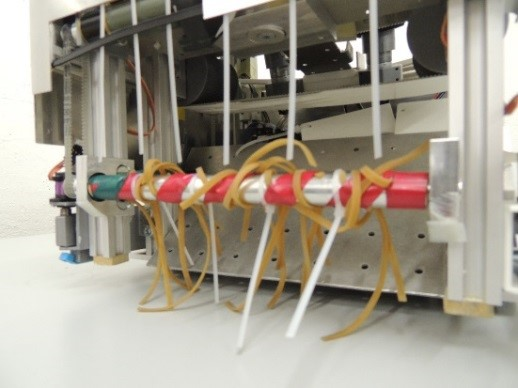
\includegraphics[width = 0.9 \textwidth]{../images/presentation/walze.jpg}
			\end{figure}
			\vspace{-2.2em}
			\begin{figure}[h]
				\centering
				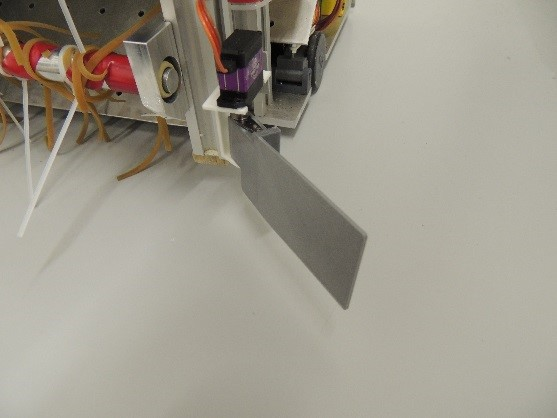
\includegraphics[width = 0.9 \textwidth]{../images/presentation/leitplanke.jpg}
			\end{figure}
		\end{column}
	\end{columns}
\end{frame}

\begin{frame}
	\frametitle{Grosser Roboter}
	\framesubtitle{Riemen und Abstreifvorrichtung}
	\begin{columns}
	\begin{column}{0.6 \textwidth}
		\begin{itemize}
			\item Beförderung zum Schussmechanismus
			\item Klebeband
			\item mechanischer Abstreifer
			\item \textit{Titanium Ores} von \textit{Moon Rocks} trennen
		\end{itemize}
	\end{column}
	\begin{column}{0.4 \textwidth}
		\vspace{-2.5em}
		\begin{figure}[h]
			\centering
			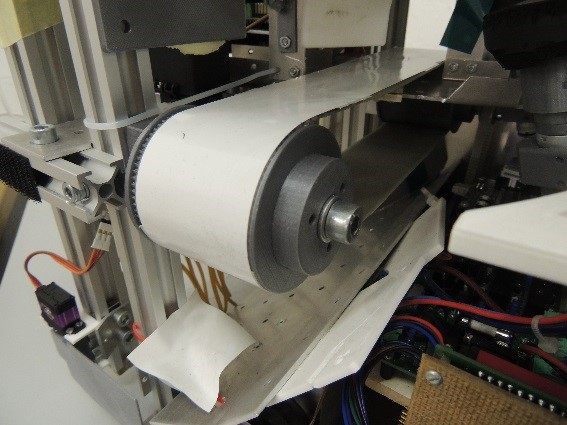
\includegraphics[width = 0.9 \textwidth]{../images/presentation/riemen.jpg}
		\end{figure}
		\vspace{-2.2em}
		\begin{figure}[h]
			\centering
			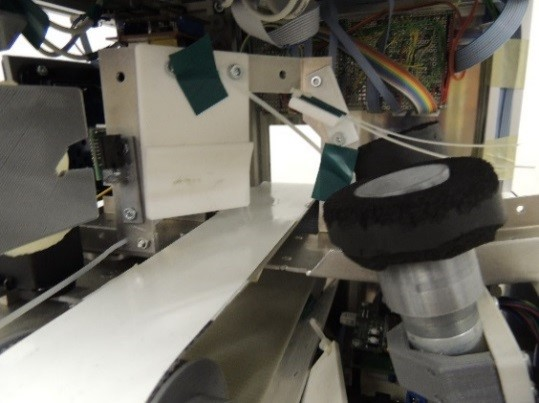
\includegraphics[width = 0.9 \textwidth]{../images/presentation/abstreifvorrichtung.jpg}
		\end{figure}
	\end{column}
\end{columns}
\end{frame}

\begin{frame}
	\frametitle{Grosser Roboter}
	\framesubtitle{Schussmechanismus}
		\begin{columns}
		\begin{column}{0.42 \textwidth}
			\begin{itemize}
				\item schiesst \textit{Titanium Ores} in die \textit{Cargo Bay}
				\item zwei sich drehende Rollen
				\item variable Distanz und Richtung
				\item Berechnung anhand der Position
			\end{itemize}
		\end{column}
		\begin{column}{0.58 \textwidth}
			\vspace{-2.8em}
			\begin{figure}[h]
				\centering
				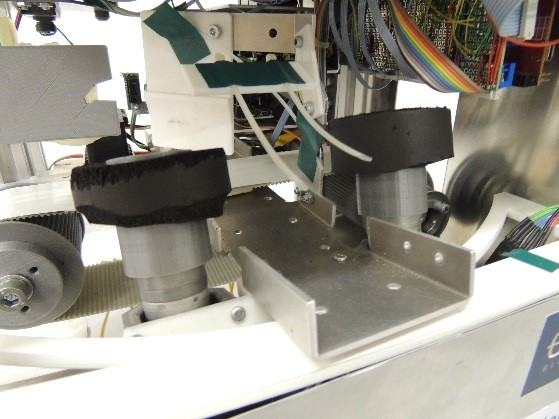
\includegraphics[width = 1 \textwidth]{../images/presentation/schussmechanismus.jpg}
			\end{figure}
		\end{column}
	\end{columns}
\end{frame}

\subsection{Kleiner Roboter}

\begin{frame}
	\frametitle{Kleiner Roboter}
	\framesubtitle{Modulaufnahme}
	Mithilfe eines Scherenzugs sollten die \textit{Lunar Modules} aus den Raketen gezogen werden.
	Dieses Konzept funktionierte nicht wunschgemäss und wurde deshalb durch einen Greifer und einen Pressfinger ersetzt.\\
	
	\begin{figure}
		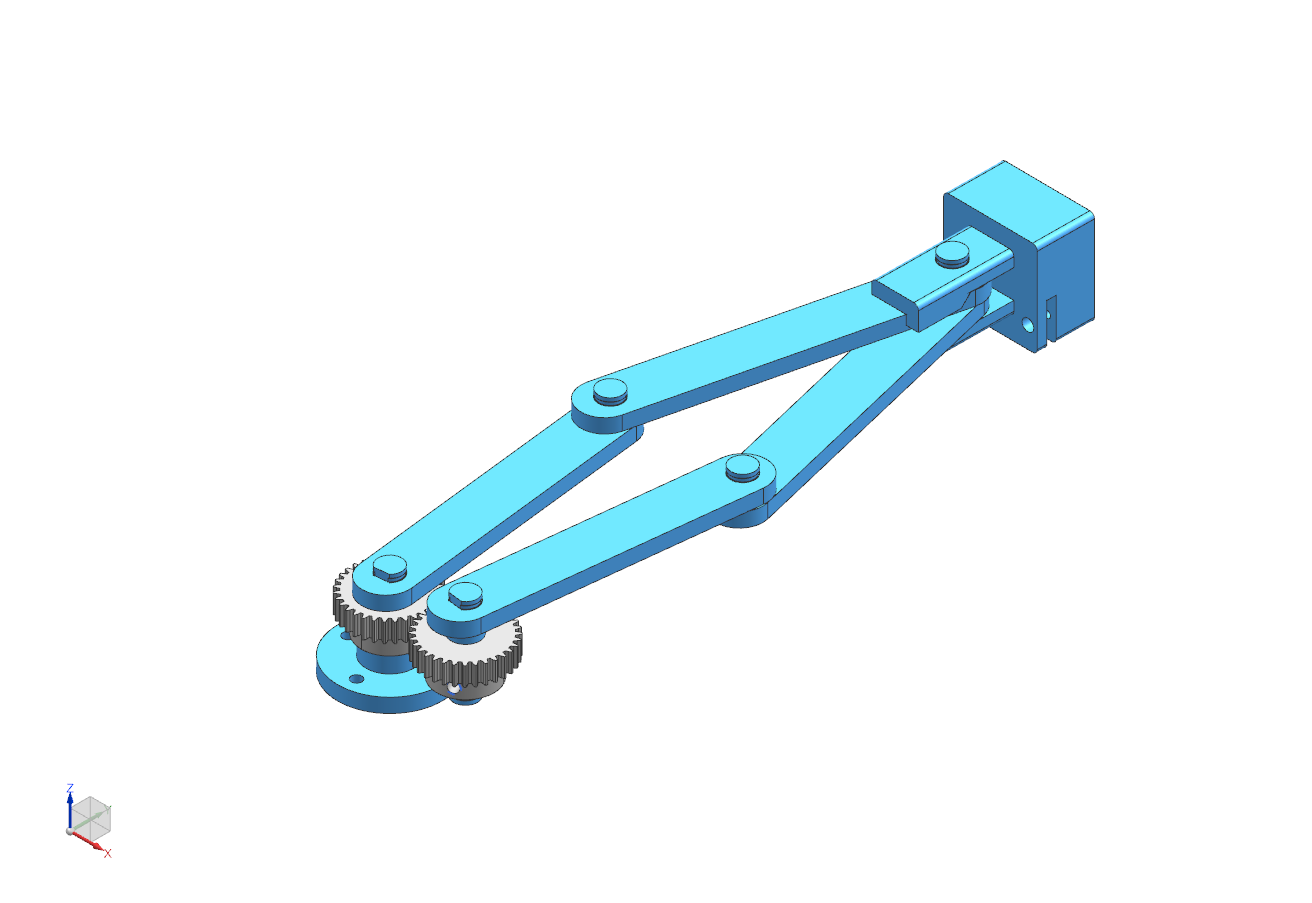
\includegraphics[height = 3 cm]{../images/presentation/kleinerRoboter/Schere.png}
		\hspace{1em}
		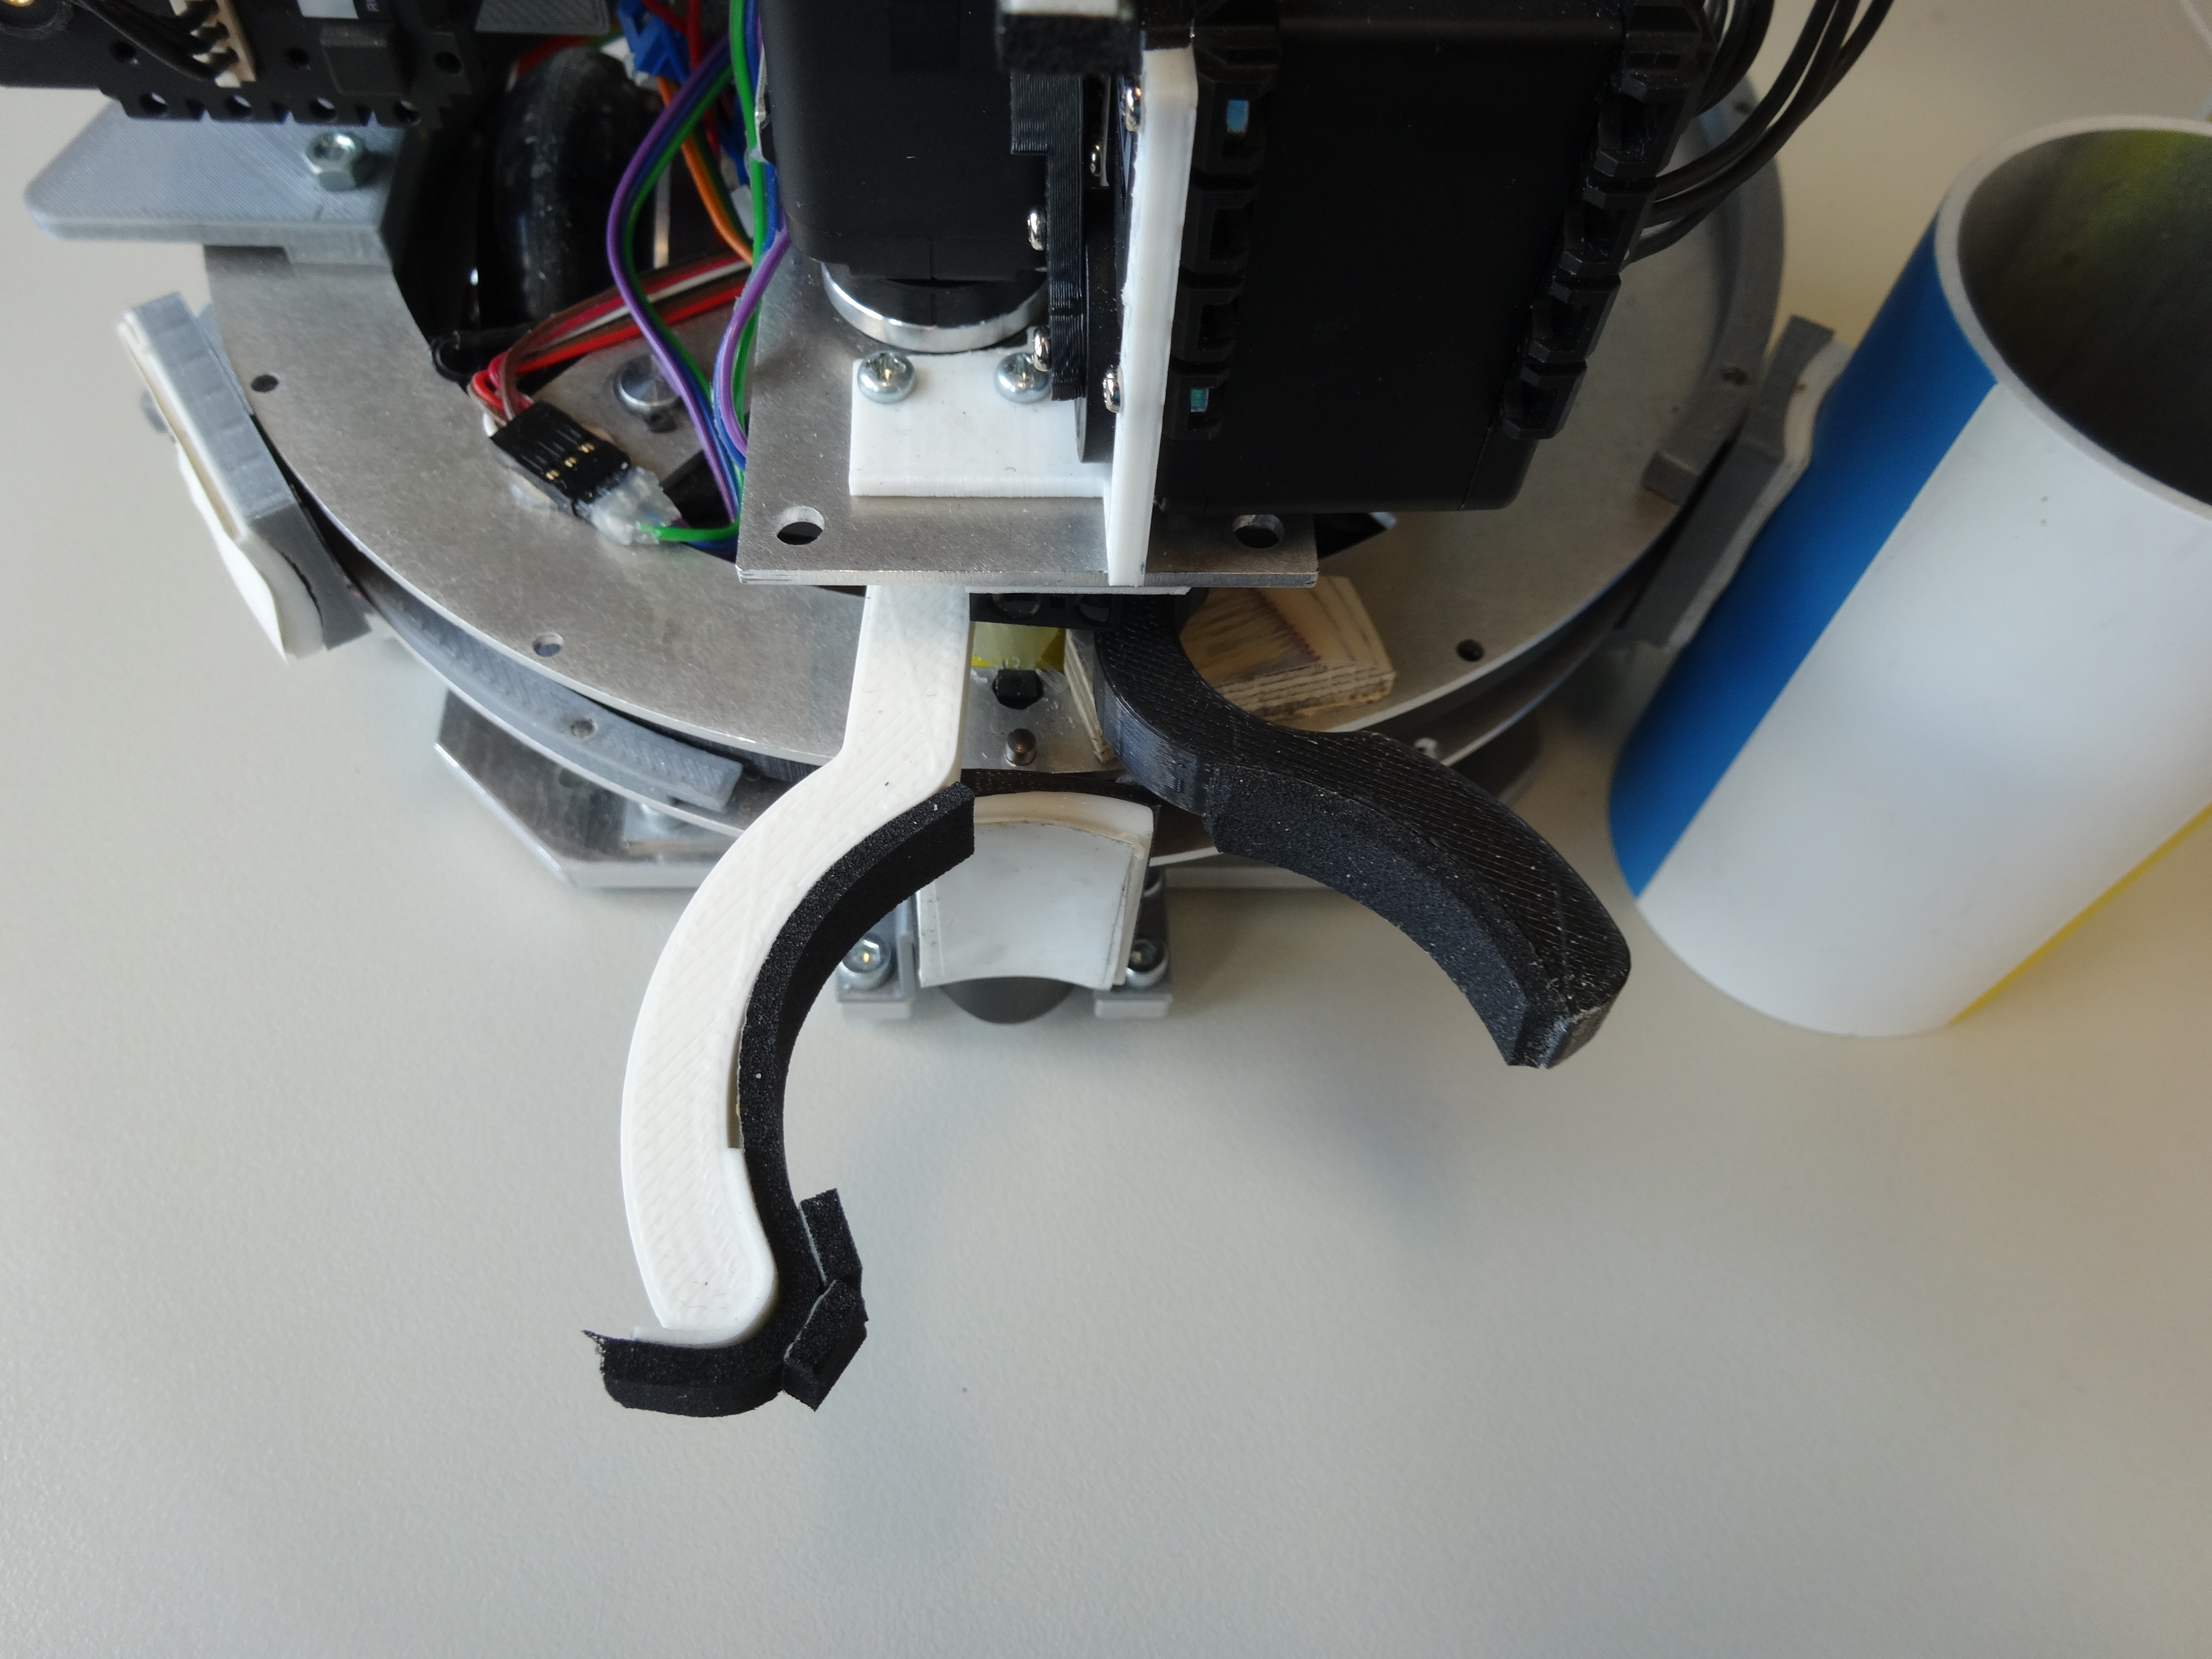
\includegraphics[height = 3 cm]{../images/presentation/kleinerRoboter/Greifer.jpg}
		\hspace{2em}
		\includegraphics[angle = 90, height = 3 cm]{../images/presentation/kleinerRoboter/Pressfinger.jpg}
	\end{figure}
\end{frame}

\begin{frame}
	\frametitle{Kleiner Roboter}
	\framesubtitle{Ring}
	Die \textit{Lunar Modules} haften während dem Transport an den Klebestellen des Rings.
	Durch drehen des Rings werden sie gekippt und abgestreift.
	\begin{figure}
		\centering
		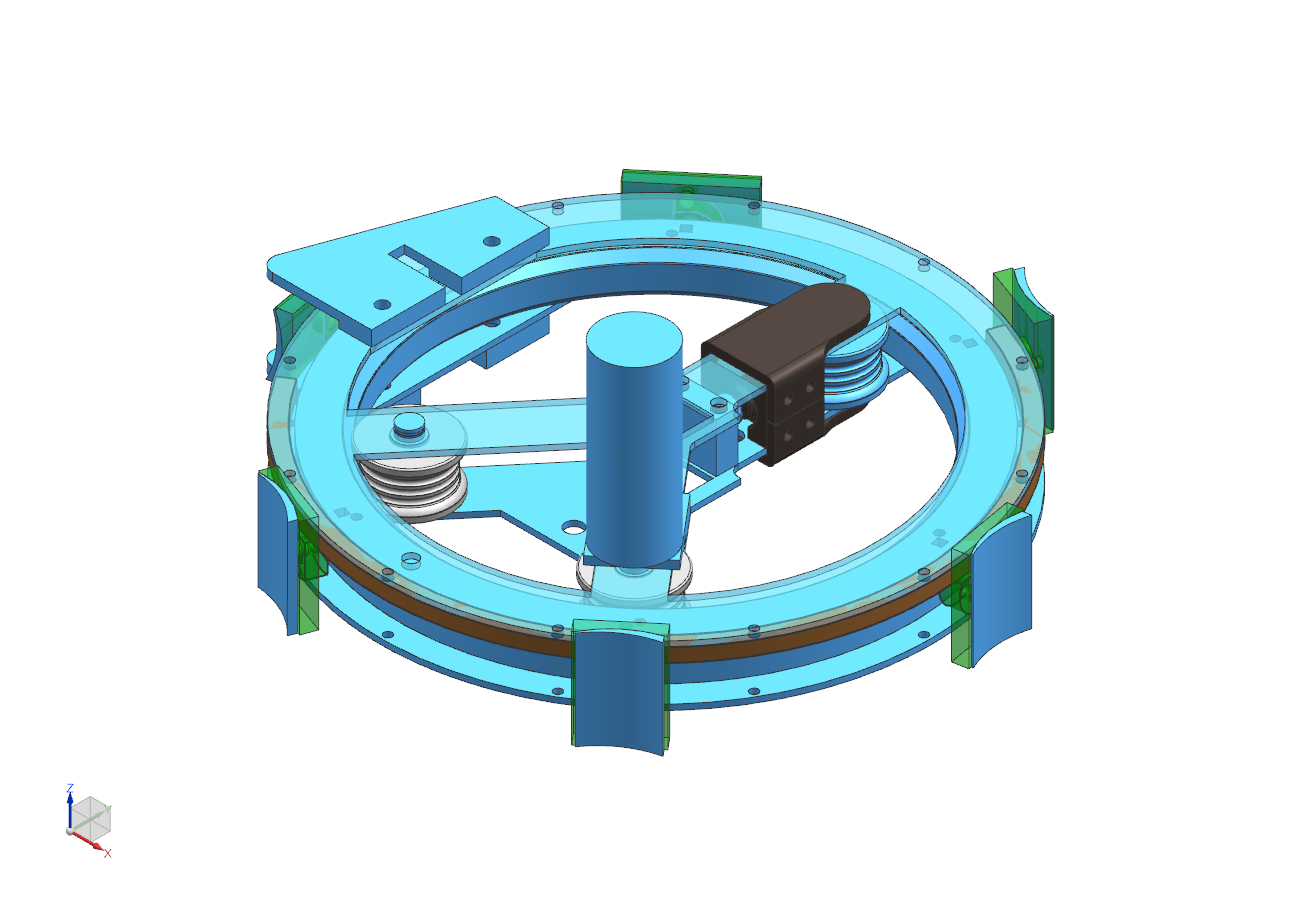
\includegraphics[height = 4 cm]{../images/presentation/kleinerRoboter/Ring.png}
	\end{figure}
\end{frame}

\begin{frame}
	\frametitle{Kleiner Roboter}
	\framesubtitle{Drehmechanismus}
	Ein Arm mit einem Farbsensor und einem Rad kann ausgeklappt werden um \textit{Lunar Modules} zu drehen oder zu verschieben.
	\begin{figure}
		\centering
		\includegraphics[height = 4 cm]{../images/presentation/kleinerRoboter/Drehen.jpg}
	\end{figure}
\end{frame}